\chapter{系统框架介绍}\label{chap:framework}
\section{引言}
本文的研究采用基于特征的视觉SLAM框架ORB-SLAM2作为基础SLAM解决方案,以提供位姿估计和几何建图功能。同时,结合了实例级的语义
分割网络Mask R-CNN,对输入的彩色图像进行预测,同步得到目标检测和像素级语义分割结果。在语义建图方面,采用了PCL点云库\citep{rusu20113d}
进行物体级的三维点云地图的构建。本章将介绍本文所研究系统的各基础部分的原理与及结构,并给出系统的整体框架描述。
\section{基于特征的视觉SLAM框架}
\subsection{视觉SLAM综述}
基于特征的视觉SLAM通过视觉传感器获取的数据流,表示为$\mathbb{F}=\left\{F_{0},...,F_{k},...,F_{N}\right\}$,
在时刻$k$,$F_{k}$表示第$k$帧的输入,可能包括彩色图$C_{k}$和深度图$D_{k}$。SLAM系统的基本任务是
估计相机的位姿和路标点集合,相机位姿为每个时刻相机自身相对于世界坐标系的转移矩阵,可表示为$\mathbb{T}=\left\{T_{0},...,T_{k},...,T_{N} \right\}$,
其中,$T_{k}$表示第$k$帧相机位姿,记为:
$$T_{k}=
\begin{gathered}
\begin{bmatrix} R_{k} & t_{k} \\ 0 & 1 \end{bmatrix}
\end{gathered}
$$
$R_{k}\in SO\left(3\right)$,表示此帧的旋转矩阵,$t_{k}\in \mathbb{R}^{3x1}$,表示此帧的平移向量。实际运算过程中,SLAM系统常常
先推算得出相邻帧$F_{k-1}$与$F_{k}$之间的转移矩阵,表示为:
$$T_{k-1,k}=
\begin{gathered}
\begin{bmatrix} R_{k-1,k} & t_{k-1,k} \\ 0 & 1 \end{bmatrix}
\end{gathered}
$$
其中$R_{k-1,k}\in SO\left(3\right)$,表示相邻阵间的旋转矩阵,$t_{k-1,k}\in \mathbb{R}^{3x1}$,表示相邻帧间的平移向量。
第$K$帧的位姿转移矩阵可以由$k-1$的位姿和两帧间的转移矩阵计算得出:
$$T_{k}=T_{k-1,k}T_{k-1}$$,而初始帧的位姿$T_{0}$常常由用户初始化为世界坐标系原点。

SLAM系统的另一项任务是估计路标点在世界坐标系中的坐标,路标点的集合可以表示为$\mathbb{L}=L_{0},...,L_{k},...,L_{M}$,
其中第$k$个路标点可以表示为$L_{k}=(x_{k},y_{k},z_{k})$。

一个完整的视觉SLAM系统可以在未知场景中同步解决以上两个问题,如图\ref{fig:SLAMflow}所示,其框架一般来说主要包括传感器数据读取、视觉里程计、后端优化、回环检测、
地图构建五个部分。具体流程为,首先由视觉传感器获取对于场景的观测信息,由视觉里程计模块负责进行帧间特征提取与匹配,完成对于相机位姿和路标点在全局坐标系下的初步估计,
得到相机轨迹和三维路标点坐标。后端模块会对系统的状态变量进行优化,得到全局最优的估计值。同时,同步运行回环检测模块,
以解决前端模块中出现的累积漂移误差。最终通过地图构建模块,生成可视化的三维地图。下面将逐模块详细介绍其工作原理。
\begin{figure}[!htbp]
    \centering
    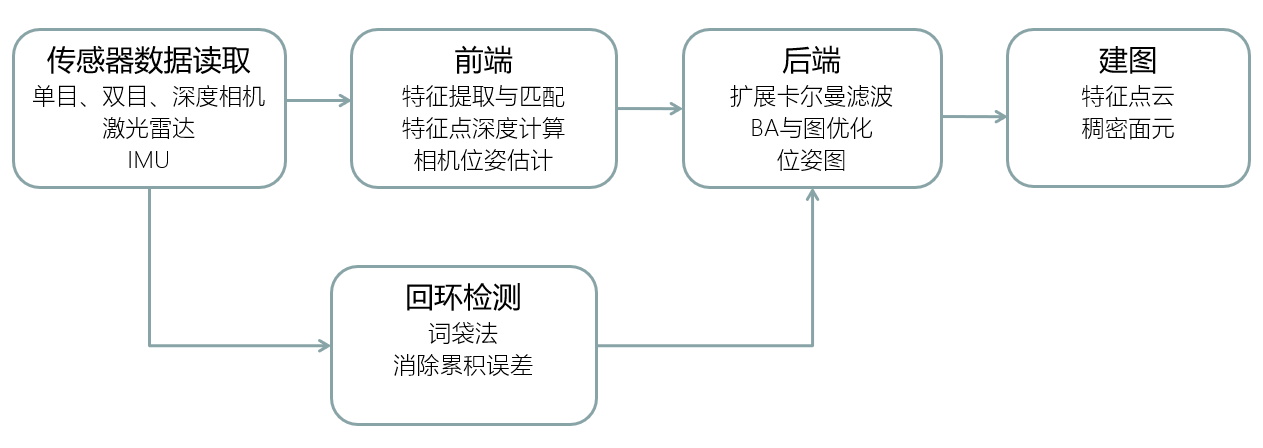
\includegraphics[width=\textwidth]{Img/2-SLAMflow.png}
    \bicaption{典型SLAM系统结构。}{Typical SLAM system architecture.}
    \label{fig:SLAMflow}
\end{figure}
\subsubsection{传感器数据读取}
视觉SLAM系统仅通过相机作为传感器来捕捉环境信息,它随着设备的移动,以恒定帧率进行拍摄,形成视频流作为系统输入。根据相机工作方式,
所用相机可以分为单目相机、双目相机、RGB-D相机三种。

其中单目相机仅有一个摄像头,其工作原理比较简单,但若想通过单目相机的数据恢复场景三维结构,必须通过移动过程中拍摄的连续帧图像,
根据视角变换造成的视差变化推测真实物体的相对距离。但单目相机仍存在尺度不确定性,通过单目相机观测数据估计的相机轨迹和三维地图
都将与真实值相差一个尺度因子。

与单目相机相比,双目相机增设了一个摄像头,通过两个摄像头同时进行拍摄,形成了天然的视差,两个摄像机之间的距离称作基线(Baseline),
通过已知的基线,可以恢复场景三维场景,消除尺度不确定性。但双目相机于单目相机都存在一个问题,即在计算路标点三维坐标时,
依赖于三角化算法以获取深度,需要大量的计算资源。

RGB-D相机使用了不同的深度值获取算法。它主要依靠相机的物理原件,如红外摄像头,激光发射器等,通过结构光或ToF(Time-of-Flight)
技术直接测量出场景中物体距离相机的距离。通过物理测量方法,可以节省大量的计算资源,但目前大多数RGB-D相机仍存在对光照变化敏感、
测量范围小等问题,因此更多用于室内场景。

\subsubsection{视觉里程计}
视觉里程计又称作前端模块,它的任务是估计相邻帧之间描述相机运动的转移矩阵和当前帧可见的路标点的三维坐标,以形成相机位姿轨迹
并构造局部地图。对于基于特征的视觉SLAM系统来说,前端模块的实现主要基于特征点法,它的思路是从每帧图像中提取能够描述局部特征的特征点,
这些特征点在相机视角发生变化后能够保持稳定,可以计算出匹配的特征点集。在传统图像处理领域,研究者们提出了多种方法来描述图像
局部特征,如SIFT\citep{LoweDistinctive}、SURF\citep{Bay2006SURF}、ORB\citep{Rublee2012ORB}等。目前由于计算资源的限制,
提取并匹配SIFT和SURF特征点无法满足SLAM系统的实时性需求,而ORB特征点成为了一个可用的选择。
ORB(Oriented FAST and Rotated BRIEF)特征是一种具有旋转不变性和尺度不变性的快速特征提取和描述方法,它分为负责特征提取的oFast
和负责特征描述的rBRIEF两部分。oFAST由FAST关键点改进得到,FAST的核心思想是以与邻域内灰度相差较大的点为关键点,oFAST在此基础上
引入了尺度金字塔,计算不同尺度上的FAST关键点。同时,oFAST还使用矩描述FAST关键点的方向,为其引入了旋转不变性。对于一FAST关键点$P(x,y)$,矩$m$的定义为:
$$m_{pq}=\sum_{x,y \in r} x^{p}y^{q}I(x,y)$$
其中$I(x,y)为$该点灰度值。该关键点的方向角$\theta$为:
$$\theta =arctan\left(\frac{m_{01}}{m_{00}}/\frac{m_{10}}{m_{00}}=arctan(\frac{m_{01}}{m_{10}})\right)$$

rBRIEF则由BRIEF描述子演化而来,BRIEF对关键点周围一定数目的点对进行灰度值比较,根据其大小关系生成二进制串作为描述符,具有匹配
速度快的特点。rBRIEF在此基础上,以关键点和取点区域的形心连线来建立二维坐标系,以此增加了旋转一致性。

在视觉SLAM视觉里程计模块中,完成特征点提取及匹配后,可选择而不同算法求解相邻阵间的转移矩阵:

\emph{\textbf{2D-2D}}\\
    若连续两帧仅有2D图像上的特征点描述,则通过对极几何关系求解本质矩阵或基础矩阵,以恢复相机运动矩阵。相邻两帧之间的运动关系
    可以通过本质矩阵(Essential Matrix)描述,表示为$E$,其包含了相机的旋转和平移变换参数,以及一个未知的平移变换因子,可以表示为:
    $$E\simeq t^{X}R$$
    其中$\simeq$表示等式两侧相差一个尺度因子。$t=\left[t_{x},t_{y},t_{z}\right]$,为平移向量,而
    $$
    t^[X]=
    \begin{gathered}
    \begin{bmatrix} 0 & -t_{z} & t_{y} \\ t_{z} & 0 & -t_{x} \\ -t_{y} & t_{x} & 0 \end{bmatrix}
    \end{gathered}
    $$
    表示平移变换,而$R$为其旋转矩阵。
    对于$F_{k-1}$和$F_{k}$上在相机坐标系下匹配的两点$X_{k-1}^{i}=\left[x_{k-1}^{i},y_{k-1}^{i},z_{k-1}^{i}\right]$和$X_{k}^{i}=\left[x_{k}^{i},y_{k}^{i},z_{k}^{i}\right]$,根据极线约束可以得出:
    $${X_{k-1}^{i}}^{T}EX_{k}^{i}=0$$
    而对于在像素平面上的两匹配二维点$P_{k-1}=\left[u_{k-1}^{i},v_{k-1}^{i} \right]$和$P_{k}^{i}=\left[u_{k}^{i},v_{k}^{i}\right]$,可得它们的齐次坐标${\widetilde P_{k-1}^{i}}=\left[u_{k-1}^{i},v_{k-1}^{i},1 \right]$和${\widetilde P_{k}^{i}}=\left[u_{k}^{i},v_{k}^{i},1 \right]$。
    通过内参矩阵$K$,可以进行像素平面上齐次坐标与相机坐标系下点的转换:
    $$
    Z{\widetilde P}
    =
    Z
    \begin{gathered}
    \begin{bmatrix} u \\ v \\ 1 \end{bmatrix}
    \end{gathered}
    =
    \begin{gathered}
    \begin{bmatrix} f_{x} & 0 & c_{x} \\ 0 & f_{y} & c_{y} \\ 0 & 0 & 1 \end{bmatrix}
    \end{gathered}
    \begin{gathered}
    \begin{bmatrix} X \\ Y \\ Z \end{bmatrix}
    \end{gathered}
    =
    KX
    $$
    其中$f_{x}$、$f_{y}$为相机焦距,$c_{x}$、$c_{y}$为主点平移。
    
    相似地,对于像素平面上的匹配点,可以由基础矩阵(Fundamental Matrix)$F$表示两帧间的极线约束关系:
    $${\widetilde{P_{k}^{i}}}^{T}F{\widetilde{P_{k-1}^{i}}}^{T}={\widetilde{P_{k}^{i}}}^{T}EK^{-1}{\widetilde{P_{k-1}^{i}}}^{T}=0$$

    $E$或$F$可以通过八点法(Eight-point-algorithm)\citep{HartleyIn},\citep{LONGUET1981A}以匹配点对组构造线性方程组解出,
    进而可以通过奇异值分解(SVD)得到相机的运动$R,t$。
    
\emph{\textbf{2D-3D}}\\若连续两帧图像中有一帧特征点对应的3D空间位置已知,则可以通过PnP(Perspective-n-Point)算法估计相机运动。
它最少仅需要3对匹配点,就能构造出线性方程组,进而解出相机转移矩阵,PnP问题的解法包括P3P\citep{GaoComplete}、EPnP\citep{lepetit2009epnp}、直接线性变换(DLT)等。
此外,也可以构造重投影误差:
$$T_{k-1,k}^{*}=\mathop{argmin}\limits_{T_{k-1,k}}\frac{1}{2}\sum\limits_{i=1}^{n}\left \| P_{k-1}^{i}-\pi \left(KT_{k-1,k}X_{k}^{i}\right) \right \|^{2}$$
其中$\pi$是将相机坐标系下的点变换至像素平面上的点的变换。通过非线性优化的方法,可以最小化重投影误差,求得最优的变换矩阵。

\emph{\textbf{3D-3D}}\\若连续两帧图像特征点对应的3D空间位置都已知,则可以通过迭代最近点(Iterative Closest Point, ICP)算法对这两组具有匹配关系的三维点进行运动估计。
一般来说,ICP问题也通过非线性优化方法求解,其构造的误差为:
$$T_{k-1,k}^{*}=\mathop{argmin}\limits_{T_{k-1,k}}\frac{1}{2}\sum\limits_{i=1}^{n}\left \| \widetilde{X}_{k-1}^{i}-T_{k-1,k}\widetilde{X}_{k}^{i} \right \|^{2}$$
其中$\widetilde{X}$表示在相机坐标系下一点$X$的齐次坐标。

计算特征点对应的路标点,即其在世界坐标系下的三维坐标,可以通过三角化(Triangularization)方法,其思想是对于同一三维点在两帧
上的投影$P_{k-1}^{i}$和$P_{k}^{i}$,它们与各自相机光心所连成的直线会在三维空间中交于一点。根据这一关系,可以构造等式,通过
最小二乘法求解得到三维点的深度值。此外,若相机能够捕捉得到深度图像,则可以方便地从深度图像中获取三维点坐标,避免了三角化过程
的计算开销。

基于特征匹配的相机位姿求解方法成为特征点法,它对于系统运行时的光照、旋转和尺度变化比较鲁棒,是长久以来比较成熟的解决方案,已具
有广泛应用。然而特征点的提取和匹配环节仍是当前SLAM系统最为耗时的一个部分,此外,在如白色墙壁等纹理缺失的场景下,提取的特征点数目会急剧下降,导致跟踪失败。

近年来学者们提出了直接法,可以能够一定程度上克服特征点法的缺点。直接法的思想是不提取图像中的特征点,而是根据相邻图像之间的灰度值
差异,构造并最小化光度误差(Photometric Error),直接恢复相机的运动。然而直接法也有一定的局限,即它的前提是灰度不变假设,因此在环境亮度变化剧烈的场景下,直接法会面临失效的风险。
$$T_{k-1,k}^{*}=\mathop{argmin}\limits_{T_{k-1,k}}\sum\limits_{i=1}^{n}\left \| I_{k-1}(P_{k-1}^{i})-I_{k}(P_{k}^{i}) \right \|^{2}$$
其中,$I(P)$为一像素平面上点$P$对应的灰度值。

\subsubsection{后端优化}
后端优化模块的主要目标是最小化SLAM过程中的因噪声等原因引入的误差,让状态估计在局部或全局下最优。其优化的目标变量是整个系统的状态变量,
即相机位姿$\mathbb{T}$和路标点集合$\mathbb{L}$。在后端优化过程中,系统的状态被抽象为一个概率模型,对于变量状态不确定性的估计
则看做一个最大后验概率估计(Maximum-a-Posteriori, MAP)过程。当前广泛应用的后端优化方法主要分为基于滤波器的优化方法与非线性优化方法。

基于滤波器的方法假设了系统的马尔科夫性,即当前时刻的状态仅与上一时刻相关。在线性高斯系统中,可以通过系统运动模型确定状态变量的先验分布,
并通过观测模型得到状态变量的似然分布,而后求解最大后验概率估计,同时也是线性系统的最优无偏估计,这一过程即为卡尔曼滤波(Kalman Filtering,KF)。
而SLAM系统中的运动模型和观测模型通常为非线性函数,因此可以以泰勒展开的方法将其近似为线性的高斯分布,以应用卡尔曼滤波算法,即扩展卡尔曼滤波(Extended Kalman Filtering,EKF)。

相比基于滤波器的方法,基于非线性优化的方法有更广泛的应用。这种方法的思想是根据全局或多帧之间变量的投影、变换、匹配等关系构造不同的约束,
使用非线性优化方法最小化误差,以得到最优的估计值。通常使用的约束包括三维点到二维平面投影所构成的约束和相机位姿的变换关系构成的约束:
$$\mathop{min}\limits_{T_{0},...,T_{N},L_{0},...,L_{M}}\sum\limits_{i=1}^{N}\sum\limits_{j=1}^{M}\left \| h(T_{i},L_{j})-l_{i,j} \right \|$$
$$\mathop{min}\limits_{T_{0},...,T_{N}}\sum\limits_{i=1}^{N}\sum\limits_{j=1}^{N}\left \| T_{i}-T_{i,j}T_{j} \right \|^{2}$$
其中,$h(T_{i},L_{j})$表示将三维路标点$L_{j}$通过第$i$帧的转移矩阵投影到二维平面$F_{i}$上的变换。

\subsubsection{回环检测}
由于前端模块仅考虑相邻帧之间的关联,每一帧位姿的估计都是建立在前一帧的估计结果之上,因此在程序运行过程中,前一帧产生的估测误差
将会不可避免的累积到下一帧上,随着程序运行时间增长,这一误差将逐渐变大,整个SLAM系统变出现了累积误差。针对这一问题,回环检测模块
的目标是在相机经过之前到达过的地方时,根据对同一地点不同时刻的观测建立约束,减少系统的累积误差,得到全局一致的状态估计。

回环检测模块的关键是如何高效地判断相机当前的观测是否曾出现过,词袋法(Bag-of-Words,BoG)是一种广泛应用的解决思路,它的核心是
用向量表示图像上的特征种类,以此描述一张图像,将两张图像向量间的距离则表示图像的相似程度。在实际应用中,如何高效比较这一向量的
相似性至关重要,利用数据结构分层存储和查找可以显著提高其效率,K-mens聚类和K叉树可以将算法复杂度降到对数级别,
是一种很好的选择,图\ref{fig:kdTree}展示了经典的KD树结构。
\begin{figure}[!htbp]
    \centering
    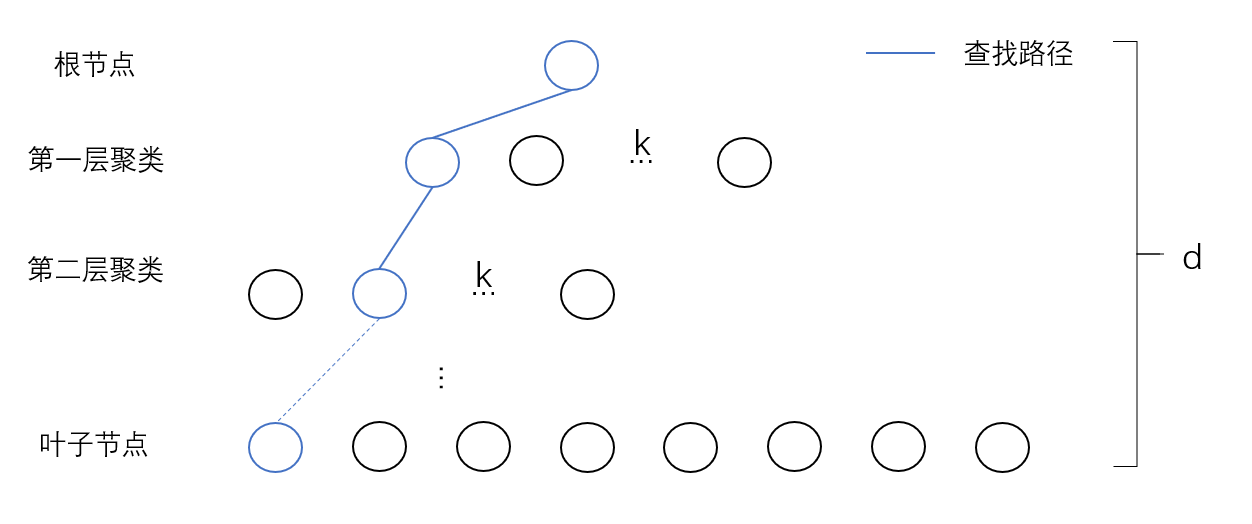
\includegraphics[width=\textwidth]{Img/2-kdTree.png}
    \bicaption{KD 树结构。}{KD tree architecture.}
    \label{fig:kdTree}
\end{figure}
\subsubsection{地图构建}
SLAM系统中地图构建模块的目标是根据已估计得到的相机位姿和路标点坐标,生成可视化的三维地图。传统SLAM生成的地图仅包含几何结构信息,
根据表示程度的不同,可以分为稠密地图和稀疏地图。建立稠密地图的方法包括TSDF建模、、面片(Surfel)模型、三角网格(mesh)建模、稠密点云、基于体素(Voxel)的八叉树模型等,
ElasticFusion是这一类别的代表工作,它融合RGB-D输入,以面片建立了室内场景地图模型。

对于基于特征的SLAM系统,更多建立的是稀疏地图,地图以路标点为单位。建立路标点首先需要在纹理丰富的关键帧中抽取特征点,经三角化或使用深度图
得到其深度信息,然后根据此关键帧的转移矩阵,将相机坐标系下的特征点变换到世界坐标系中,成为三维地图中一点。除此之外还需要
在后端优化模块对三维地图点集进行坐标优化,使其重投影误差最小化。整个地图构建模块与视觉里程计和后端优化模块环环相扣,是其对
环境感知结果的可视化表达。

\subsection{ORB-SLAM2结构简介}
ORB-SLAM2是当前最完善的基于特征的SLAM框架之一,在大多数场景下都有着出色的跟踪、建图表现和鲁棒性。本文的研究便以ORB-SLAM2为基础,
它能够接收受单目、双目、RGB-D格式的图像输入,包含位姿估计、稀疏建图、局部与全局优化、闭环检测与闭环纠正等功能,其系统分为跟踪(Tracking)、
局部地图(Local Mapping)、回环闭合(Loop Closing)三个线程,具体系统结构如图\ref{fig:orbslam}所示。
\begin{figure}[!htbp]
    \centering
    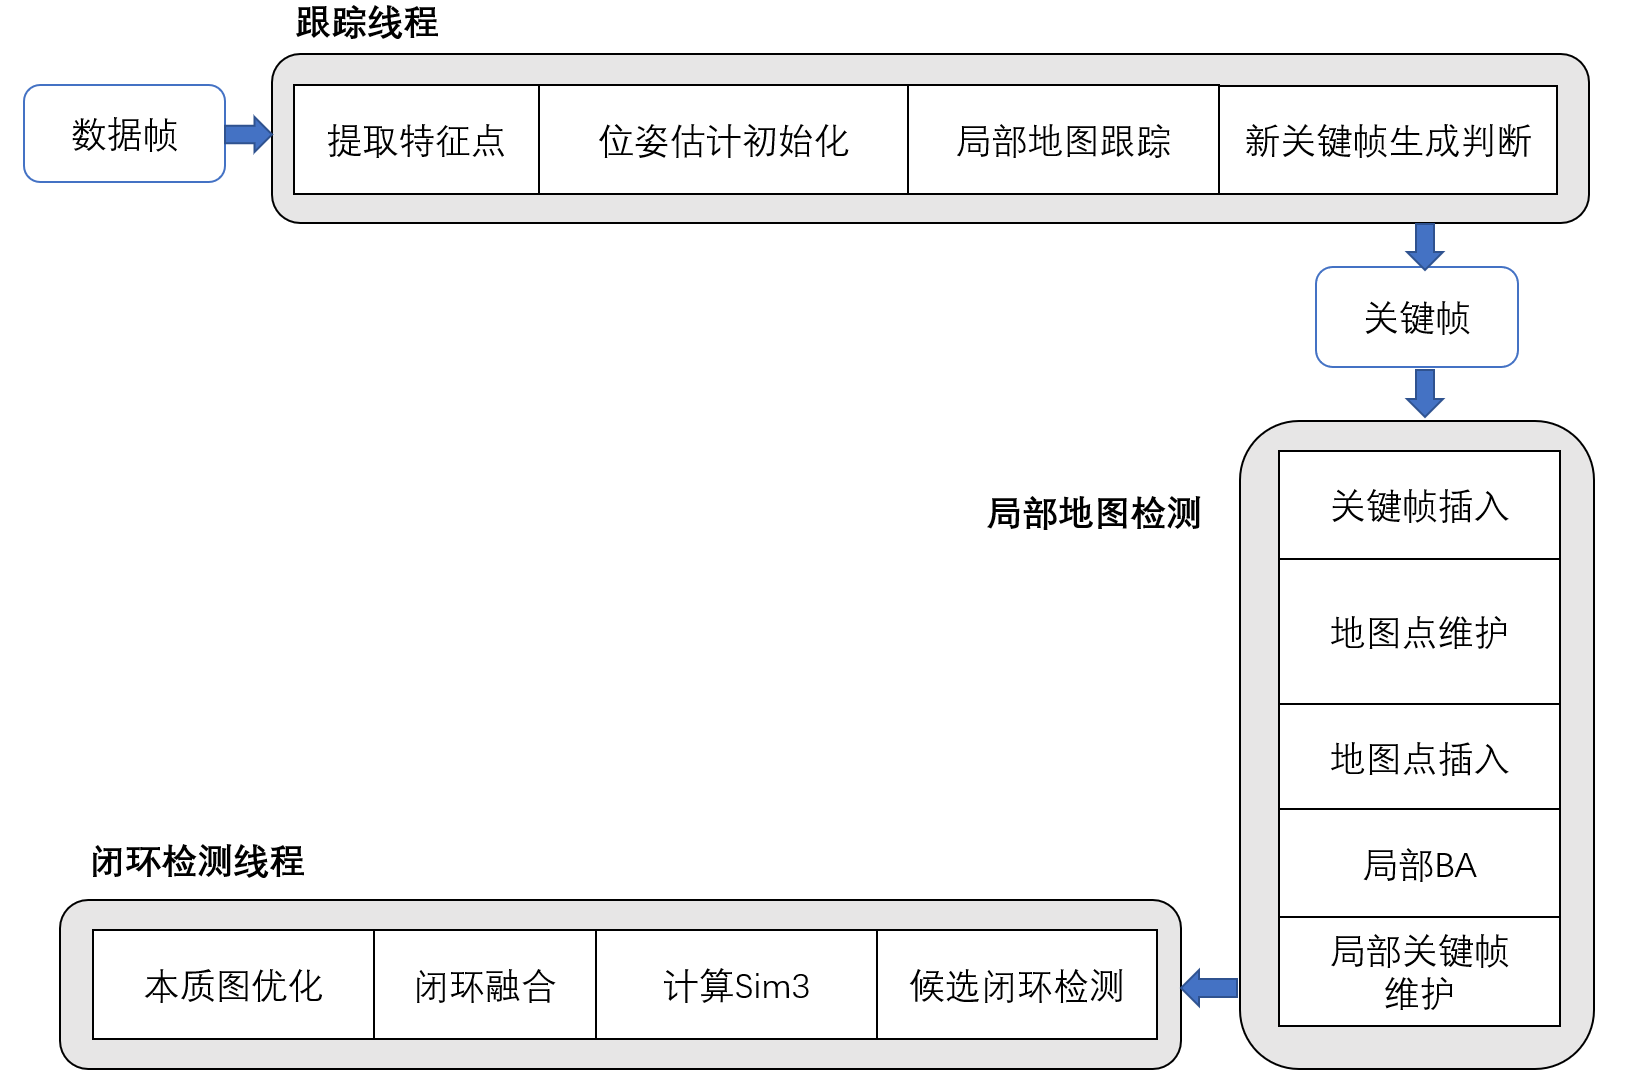
\includegraphics[width=\textwidth]{Img/2-ORBSLAM.png}
    \bicaption{ORB-SLAM2系统结构。}{System architecture of ORB-SLAM2.}
    \label{fig:orbslam}
\end{figure}
相机捕获的图像数据流首先输入跟踪线程,系统从中提取ORB特征点,在相机稳定移动的情况下根据相邻帧间特征点匹配结果,以恒速模型
初始化相机位姿的估测值,若相机运动较剧烈,也可通过参考帧或重定位的方法进行位姿初始化,这一操作也增加了系统的鲁棒性。同时,
对于单目或多目的数据输入,系统还会通过三角化算法得到特征点的深度值。之后,在当前帧的局部范围内将进行局部地图跟踪,轻量级地
进行优化。最后,在跟踪线程中还将判断并生成关键帧。

关键帧将输入局部地图线程,用于更新和维护路标点集合,并通过局部捆绑调整的方法进行优化。此外系统还维护了关键帧队列,以“宽入严留”
的方式更新关键帧集合,进一步增强了系统鲁棒性。

系统还同步运行回环闭合模块,此模块分为闭环检测和和闭环纠正两部分。在闭环检测部分,通过词袋模型来检测闭环,在发生闭环时求解Sim3,
用于在闭环纠正部分调整局部地图的位姿,并运行一次全局捆绑调整,在全局范围下进行状态估计的优化。

\section{基于深度学习的实例分割神经网络}

在深度学习飞速发展的今天,深度神经网络在各领域取得了优秀表现,包括计算机视觉、语音识别、自然语言处理等等。语义分割是计算机视觉
领域的基本任务之一,它的目标是对于图像中的每一个像素预测其所属类别,SegNet\citep{VijaySegNet}、FCN\citep{long2015fully}、DeepLab\citep{chen2018encoder}\citep{Chen2014Semantic}、U-Net\citep{ronneberger2015u}
等都是针对这一任务表现优异的网络结构。而目标检测是指针对一副输入图像,识别出其中存在的物体,输出该物体的类别、置信度以及位置框
(bounding box)。Fast R-CNN\citep{girshick2015fast}、Faster R-CNN\citep{ren2015faster}、YOLOv3\citep{redmon2018yolov3}、SSD\citep{Liu2016SSD}
等都是这一研究领域的代表工作。而实例分割结合了语义分割和目标检测的特点,能够同时输出表示像素类别标签的语义Mask和目标检测结果,
本文选用的网络结构Mask R-CNN\citep{HeMask}便是一个出色的实例分割网络。
\begin{figure}[!htbp]
    \centering
    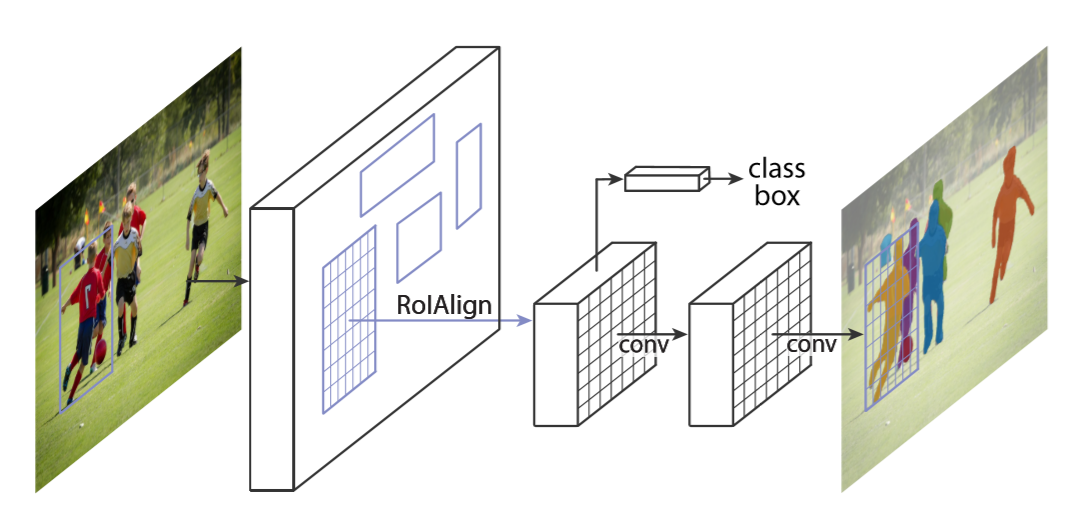
\includegraphics[width=0.5\textwidth]{Img/2-maskRCNN.png}
    \bicaption{实例分割网络Mask R-CNN。}{Instance segmentation network Mask R-CNN.}
    \label{fig:maskRCNN}
\end{figure}
Mask R-CNN以广泛应用的目标检测网络Faster R-CNN为原型,并在其基础上增加了进行语义分割任务的分支。Faster R-CNN 是一个
双阶段的目标检测方法,它包括区域候选网络(Region Proposal Networks, RPN)和位置框回归(Bounding Box Regression)两个部分。
在区域候选网络阶段,RPN将用于生成不同尺度锚框(anchor),以在特征图上对检测框进行粗略描述。对于每个锚框,分别进行前景、背景
分类和位置框的回归,输入建议层(Proposal Layer)。在建议层中,按每个锚框前景类别的Softmax得分排序,经过极大值抑制选取得分最高
的固定数目锚框,生成检测框,完成目标定位过程。不同尺度的检测框会输入兴趣区域池化层(ROI Pooling layer),得到固定大小的特征图。
随后特征图分别送入分类与回归两个分支,在分类分支中经全连接层和Softmax层得到该检测框对应各类别的概率,在回归分支中则再次进行
位置框回归,得到更加准确的位置框预测结果。
\begin{figure}[!htbp]
    \centering
    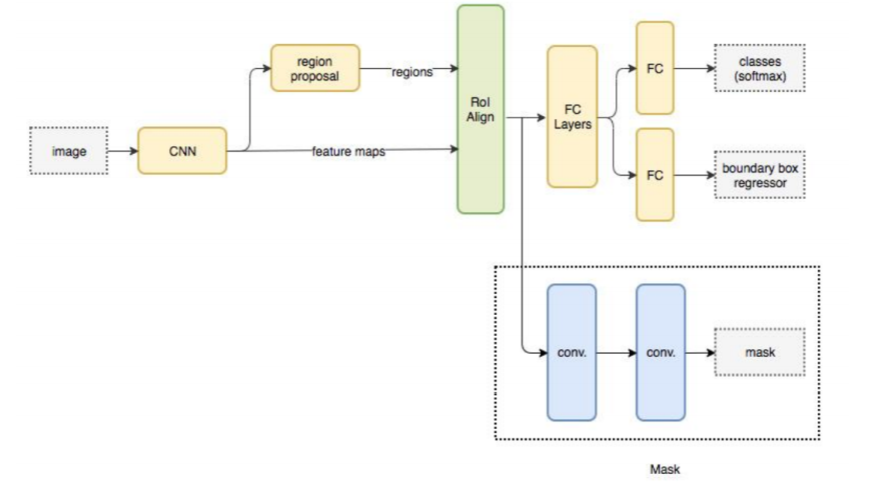
\includegraphics[width=\textwidth]{Img/2-maskRCNNStructure.png}
    \bicaption{Mask R-CNN网络结构。}{Architecture of Mask R-CNN.}
    \label{fig:maskRCNNStructure}
\end{figure}
以Faster R-CNN为基础,Mask R-CNN分为骨干网络和头部网络部分,其结构如图\ref{fig:maskRCNNStructure}所示。骨干网络部分使用ResNet-FPN\citep{he2016deep},负责特征提取。
其中特征金字塔网络(Feature Pyramid Network,FPN)是一种多尺度检测方法,它将ResNet中每个残差块不同尺度的特征图自下而上以
elewise的方式进行整合,不同尺度的特征图经上采样相加,会同时保留低层细节特征和高层全局特征,有利于不同尺度目标的检测。
同时Mask R-CNN提出了兴趣区域对齐算法(RoI Align),将不同层级的特征图输入区域候选网络,消除了兴趣区域池化层带来的的精度损失,
得到了更精准的检测结果,并能够提升分割分支的精度。头部网络部分则是在Fast R-CNN的基础上增加了分割分支,变成前景类别分类、
位置框回归和mask分割三个分支并行的结构,能够完成同步目标检测和实例分割。
\begin{figure}[!htbp]
    \centering
    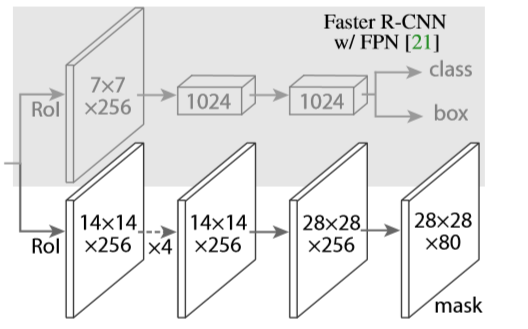
\includegraphics[width=0.35\textwidth]{Img/2-headNetwork.png}
    \bicaption{Mask R-CNN的头部网络结构。}{Network head of Mask R-CNN.}
    \label{fig:headNetwork}
\end{figure}
本文所使用的Mask R-CNN模型使用公开数据集Microsoft COCO\citep{lin2014microsoft}训练,能够检测多达80个类别的物体。
对于第$k$帧中的输入彩色图像$C_{k}$,我们可以获得两个输出:
{
\setlist[enumerate]{}% restore default behavior
\begin{enumerate}[nosep]
    \item 语义mask$m_{k}$。以张与输入图像分辨率相同的单通道图像,其中每个像素的灰度值代表该像素的类别标签。
    \item $J$个对象的检测结果集$\mathbb{R}={r_{0},...,r_{j},...r_{J}} $,其中第$j$个目标的检测结果可表示为$r_{j}={c_{j},b_{j},s_{j}}$,
    $b_{j}=\left[bu_{j},bv_{j},bw_{j},bh_{j}\right]$,每项分别代表该检测框的左上角坐标和宽度、高度。
    每一项分别代表其类别,边界框和置信度。在语义分割阶段,$s_{j}$过低的目标将被抛弃不用,以此保证每一个参与后续流程的目标检测结果
    都足够可靠,而$c_{j}$和$b_{j}$将用于后续的位姿优化及语义建图。
\end{enumerate}
}

\section{系统框架设计}
\begin{figure}[!htbp]
    \centering
    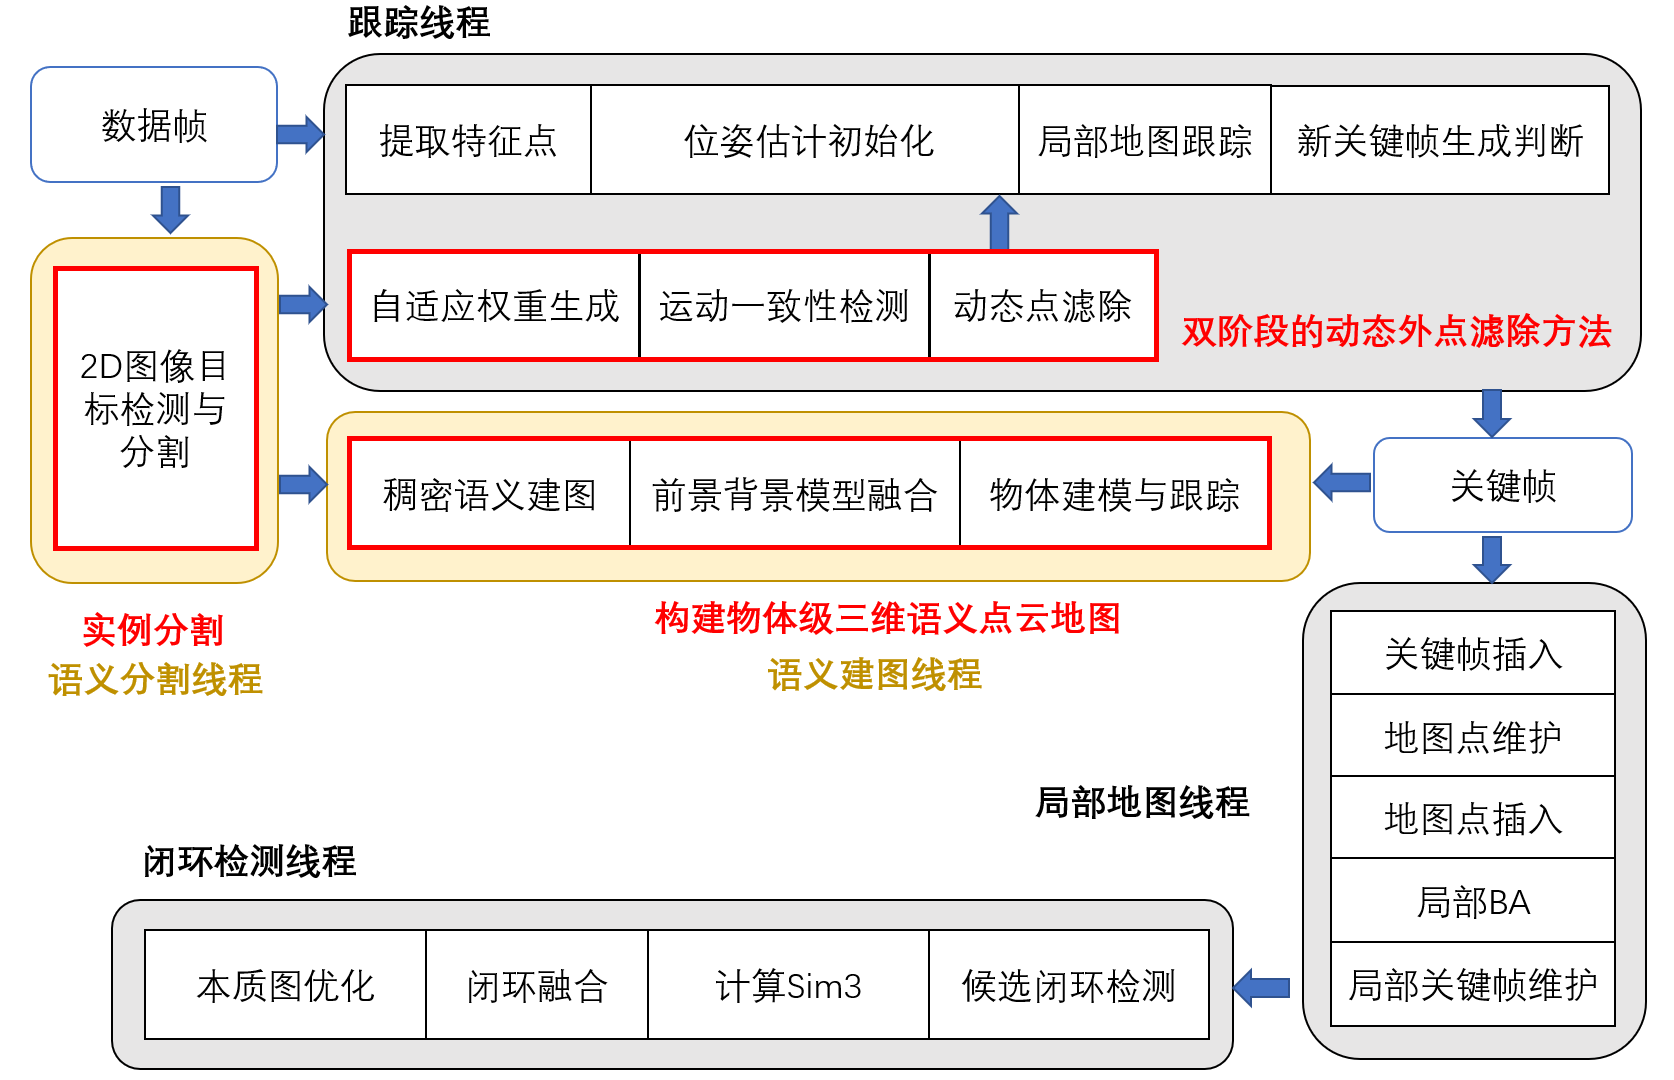
\includegraphics[width=\textwidth]{Img/2-orbPlus.png}
    \bicaption{本文所提出的基于ORB-SLAM2的系统结构。}{ORB-SLAM2-based system architecture proposed in this paper.}
    \label{fig:orbPlus}
\end{figure}
本文将所提出的系统通过深度学习框架Keras将Mask R-CNN结合在了基于特征的视觉SLAM系统ORB-SLAM2中,使得SLAM运行过程中,能够同步
对输入的图像数据进行实例分割,输出目标的类别、置信度、位置框和语义mask。相比于ORB-SLAM2,本文所提出的系统接受RGB-D输入,改进了跟踪线程
并新增了语义建图线程,系统整体共有五个平行的线程:跟踪、局部地图、语义分割、回环闭合和语义建图,具体结构如图\ref{fig:orbPlus}所示。
\begin{figure}[!htbp]
    \centering
    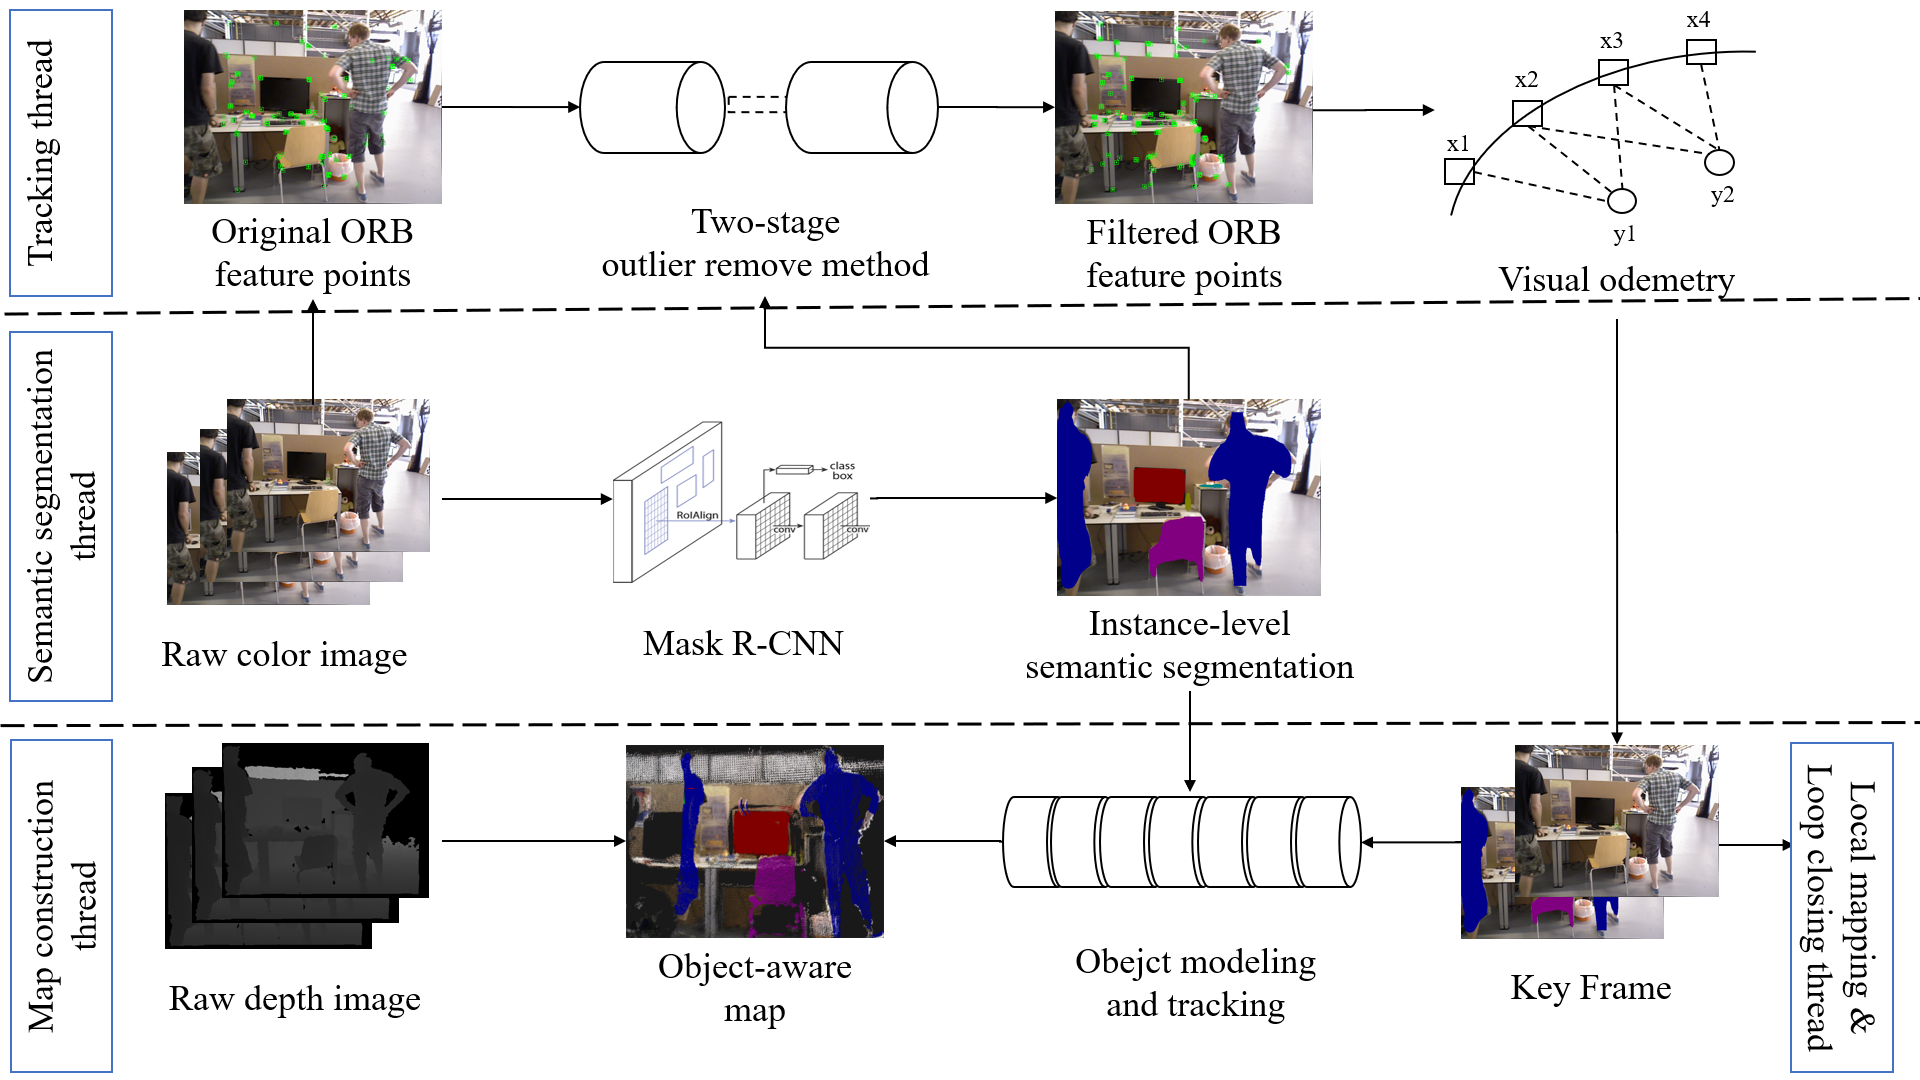
\includegraphics[width=\textwidth]{Img/2-overview.jpg}
    \bicaption{系统工作流程。}{Workflow of our system.}
    \label{fig:overview}
\end{figure}
图如\ref{fig:overview}所示,系统工作流程为:相机捕获RGB-D数据流,每一帧包含彩色图和深度图。输入的彩色图会同步用于语义分割和跟踪线程。
在跟踪线程中,系统对输入的彩色图像提取ORB特征,然后结合语义分割线程输出的预测结果,通过双阶段的动态外点滤除算法
检测动态目标并移除位于动态目标轮廓的特征点,然后对经过滤除的剩余特征点进行特征匹配,用于计算得到相机位姿和路标点估计,
同时会通过一定的策略生成关键帧,分别输入局部地图线程和语义建图线程。局部建图线程与回环闭合线程共同对状态变量进行优化,
得到全局最优的状态估计。语义建图线程会结合语义分割线程输出的预测结果,对其检测到的目标进行建模和跟踪,并随环境变化而更新,
同时会进行2D-3D语义关联,为三维地图中的物体模型赋予不同的语义标签,以建立物体级的语义点云地图。

\section{本章小结}
本章从宏观上介绍了本文的基本框架结构,力求清晰、完整地串联起本文所研究的系统的整体结构和各部分间关联。首先在第一节介绍了SLAM的基本任务和技术要点,第二节介绍了本文所研究的系统所采用的基于特征
的视觉SLAM框架——ORB-SLAM2,第三节介绍了本文所研究的系统采用的网络结构——Mask R-CNN,最后一节阐述了本文所研究系统各个模块
间的关联、交互方式,给出了系统框架设计。
